\subsection{Simulating neural activity in a neural population} \label{sec:results:simulations}

To test the described method for inferring functional connectivity from calcium imaging data, we simulated networks (according to our model, Eqs. \ref{eqn:glm:definition} -- \ref{eqn:F:definition}) of spontaneously firing randomly connected neurons.  Although simulations ran at $1$ msec time discretization, imaging rate was assumed to be much slower. Simulations lasted anywhere between 5 minutes and 1 hours (of simulated time).  Model parameters were chosen based on experimental data available in the literature
for cortical neural networks \cite{Braitenberg1998,Urquijo2000,Lefort2009,Sayer1990}.

More specifically, the network contained 80\% of excitatory and 20\% inhibitory neurons \cite{Braitenberg1998,Urquijo2000}, each respecting Dale's law. Neurons were randomly connected to each other with probability $0.1$ \cite{Braitenberg1998,Lefort2009}.  Synaptic weights for excitatory connections, as defined by EPSP peak amplitude, were randomly drawn from exponential distribution with the mean of $0.5 \mu V$ \cite{Lefort2009,Sayer1990}.
Inhibitory connections were also drawn from exponential distribution; their strengths chosen so as to balance excitatory and inhibitory currents in the network, and achieve an average firing rate of  $\approx 5 $ Hz \cite{Abeles01}. Practically, this meant that the mean strength of inhibitory connections was about 10 times larger than that of the excitatory connections.

Note that EPSP peak amplitudes cannot be used directly in Eq. \ref{eqn:glm:definition}. Really, $w_{ij}$ in Eq. \ref{eqn:glm:definition} is a dimensionless quantity representing the change in the spiking probability of neuron $i$ given neuron $j$ fired, while EPSP peak amplitude describes physiologically measured change in the membrane voltage of a neuron due to synaptic currents triggered by spike in neuron $j$. These two quantities, therefore, are dramatically different and we need to find a way to relate the two.

For that, we first point out that in order to trigger an immediate spike in a neuron that typically has its membrane voltage $V_b$ $\mu$V below the spiking threshold $n_E = V_b / V_E$ simultaneous EPSPs with the peak amplitude $V_E$ would be necessary.
Therefore, we propose that the change in the spiking probability of a neuron due to excitatory synaptic current $V_E$ can be approximately defined as
(so that $\delta P_E n_E \approx 1$)
\begin{equation}\label{eqn:convert:leadin-1}
\delta P_E = V_E/V_b.
\end{equation}
At the same time, according to Eq. \ref{eqn:glm:definition}, the same change in the spiking probability of a neuron $i$ following the spike of a neuron $j$ should be defined in GLM as
\begin{equation}\label{eqn:convert:leadin-2}
\delta P_E = \exp[-e^{b_i+w_{ij}}\tau_w]-\exp[-e^{b_i}\tau_w]
\end{equation}
Here $\tau_w$ is the typical EPSP time-scale, i.e. the time over which EPSP of one neuron, $j$, significantly affects the firing probability of the other neuron, $i$.

Equating Eq. \ref{eqn:convert:leadin-1} and Eq. \ref{eqn:convert:leadin-2}, we arrive at the proposition for our link function for physiologically measured EPSP peak amplitude, $V_E$, and GLM weight, $w_{ij}$:
\begin{equation}\label{eqn:convert}
\w_{ij}=\ln(-\ln(e^{-r_i\tau_w}-V_E/V_b)/r_i\tau_w).
\end{equation}
Here $r_i=\exp(b_i)$ is the base firing rate of neuron $i$. PSP shapes were modeled as an alpha function \cite{Koch99}, by differencing of two exponentials, corresponding to a sharp rise and relatively slow decay \cite{Sayer1990}.
%The time course of functional connectivity weights $\w_{ij}(t)$ was modeled as the difference of two exponentials, resulting in a rise time of $\tau_r=1$ msec and decay time of $\tau_{E_d}=10$ msec for excitatory and $\tau_{I_d}=20$ msec for inhibitory currents . In practice, we sampled time constants from uniform distributions with means as stated above and support of $\pm 25 \%$ of the means.
We neglected conduction delays, given that the time delay below $\sim 1$ msec expected in local cortical circuit was smaller than the time step of our computer simulation.  Each neuron also had an exponential refractory current \cite{Koch99}.

Parameters for the internal calcium dynamics and fluorescence observations were chosen according to our experience with several cells analyzed using algorithm of \cite{Vogelstein2009}, and conformed to other experimental observations \cite{ImagingManual,HelmchenSakmann96,BrenowitzRegehr07}. Each parameter was generated from a normal distribution with specified mean and variance at about 30\% of the mean, truncated at the lower bound at about 30\% of the mean value.  Table \ref{table:caparm} summarizes the details for each of the parameters in our model.

\begin{table}[h!b!p!]
\caption{Table of simulation parameters. $\mathcal{E}(\lambda)$ indicates an exponential distribution with mean $\lambda$, and $\mathcal{N}_p(\mu,\sigma^2)$ indicates a normal distribution with mean $\mu$ and variance $\sigma^2$, truncated at lower bound $p\mu$.}\label{table:caparm}

\begin{tabular}{ll}
\hline
Total neurons & 10-500 \\
Excitatory neurons & $80\%$ \\
Connections sparseness & $10\%$ \\
Baseline firing rate & 5 Hz\\
\hline
EPSP peak height 	& $\sim \mathcal{E}[0.5 \mu$V] \\
IPSP peak height 	& $\sim \mathcal{E}[2.3 \mu$V] \\
EPSP rise time 		& 1 msec \\
IPSP rise time 		& 1 msec \\
EPSP decay time 	& $\sim \mathcal{N}_{0.5}[10 $ msec$,(2.5 $ msec$)^2]$ \\
IPSP decay time 	& $\sim \mathcal{N}_{0.5}[20 $ msec$,(5 $ msec$)^2]$ \\
refractory time 	& $\sim \mathcal{N}_{0.5}[10 $ msec$,(2.5 $ msec$)^2]$ \\
\hline
Calcium std. $\sigma_c$ & $\sim \mathcal{N}_{0.4}[28\mu$M$,(10\mu$M$)^2]$ \\
Calcium jump after spike, $A_c$ &  $\sim \mathcal{N}_{0.4}[80\mu$M$,(20\mu$M$)^2]$\\
Calcium baseline, $C_b$ & $\sim \mathcal{N}_{0.4}[24\mu$M$,(8\mu$M$)^2]$ \\
Calcium decay time, $\tau_c$ & $\sim \mathcal{N}_{0.4}[200 $ msec$,(60 $ msec$)^2]$ \\
Mean photon budget $\alpha_c$ & $1$--$80$ Kph/neuron/frame \\
Dissociation constant, $K_d$ & $200 \mu$M \\
\hline
\end{tabular}
\end{table}


\subsection{Inferring functional connectivity from the simulated calcium imaging data} \label{sec:results:inference}

With neural population activity prepared as described in the previous section, we used our inference algorithms to reconstruct the functional connectivity matrix from simulated fluorescence data. Specifically, we estimated the connectivity matrix using both
the embedded-chain-within-blockwise-Gibbs approach as well as factorized approximation, Figure \ref{fig:scatters}.  We found that factorized approximation was able to provide reconstructions almost as accurate as the exact embedded-chain-within-blockwise-Gibbs approach --- $r^2=0.47$ versus $r^2=0.48$ --- when parameters corresponded to a realistic preparation, given $10$ minutes of simulation data, and a population of $N=25$ neurons.
We furthermore estimated the weights using GLM from the true spike trains, and the
true spike trains down-sampled to the frame rates  of calcium imaging,
$r^2=0.7$ and $r^2=0.57$ respectively.
thus, the quality of our estimates using the fluorescence traces was worse than those obtained from the the true down-sampled spike trainsm
although for SNR of fluorescence data the $r^2$ values for obtained reconstructions approached that of down-sampled true spike trains, Figure \ref{fig:recvar-SNR}.
Example of what we understand by high SNR (can be used for functional connectivity
inference) and low SNR (cannot be used for functional connectivity inference)
are shown in Figure \ref{fig:recvar-SNR} on two fluorescence traces from real
in-vivo data.

%Fluorescence data is generally acquired at low frame rate and, so, one of its main limitations is bad time-resolution of the observed spike trains. To determine the impact of this constraint on the connectivity reconstructions, and, thus, to determine how close calcium imaging may approach reconstructions from spike trains directly observed under comparable conditions, we conducted this experiment. We observed that at intermediate SNR reconstructions from calcium imaging closely resembled such obtained directly from spike trains, and at higher SNR reconstruction with the quality same with original spike trains was achieved, Figure \ref{fig:scatters} and \ref{fig:recvar-SNR}.


%\begin{align}
% \label{eqn:likelihoodGLMmoda}
% &E[\ln P[n_i(t)| \bh(t); b_i, k_i, \bw_i, S(t)]
% 	=\sum_t \left( n_i(t) \ln J_i(t) - (1-n_i(t)) \exp(J_i(t)) \Delta \right), \\
% \label{eqn:likelihoodGLMmodb}&J_i(t)=b_i+\sum\limits_j \sum\limits_{t'<t} \w_{ij}(t-t')n_{j}(t')=
% b_i+\sum\limits_j w_{ij} h_j(t).
% \end{align}

\comment{The sum in Eqs.\ref{eqn:likelihoodGLMmoda} and \ref{eqn:likelihoodGLMmodb} was over the sample of $\{n_i(t)\}$, produced with our spike sampling algorithm, discretized over the time-bins $t'$ with the width corresponding to the calcium imaging frame rate (i.e. 30 ms for 33 Hz and 15 ms for 66 Hz). In one of the two cases we considered, EPSP time-profiles were assumed to be ``known'' exponential, and the weights were estimated using reduced histories $h_{i}(t)=\sum_{t'<t} \exp(-(t-t')/\tau_h)n_{i}(t')$ with the time constant $\tau_h=10$ ms (i.e. second equation in Eq. \ref{eqn:likelihoodGLMmodb}). In the second case we considered, the time dependence of $\w_{ij}(t)$ was assumed to be unknown and the first equation in Eq. \ref{eqn:likelihoodGLMmodb}) was used to correlate $n_i(t)$ with $n_j(t')$ for $t'<t$ up to a given depth $m$.  In this latter case, since each next term in Eq. \ref{eqn:likelihoodGLMmodb}) was significantly smaller than the previous one, we found that the best results were obtained if we took $m=1$ (i.e. minimizing number of unknown variables given certain amount of data).
In either case, we described the connection weight between two neurons by a scalar quantity $w_{ij}^s=\text{sign}(\w_{ij})\max_{t} |\w_{ij}(t)|$, which thereafter was used to compare true and reconstructed connectivity weights in all examples below.}

\begin{figure}[h]
\centering
\begin{minipage}[c]{0.45\hsize}
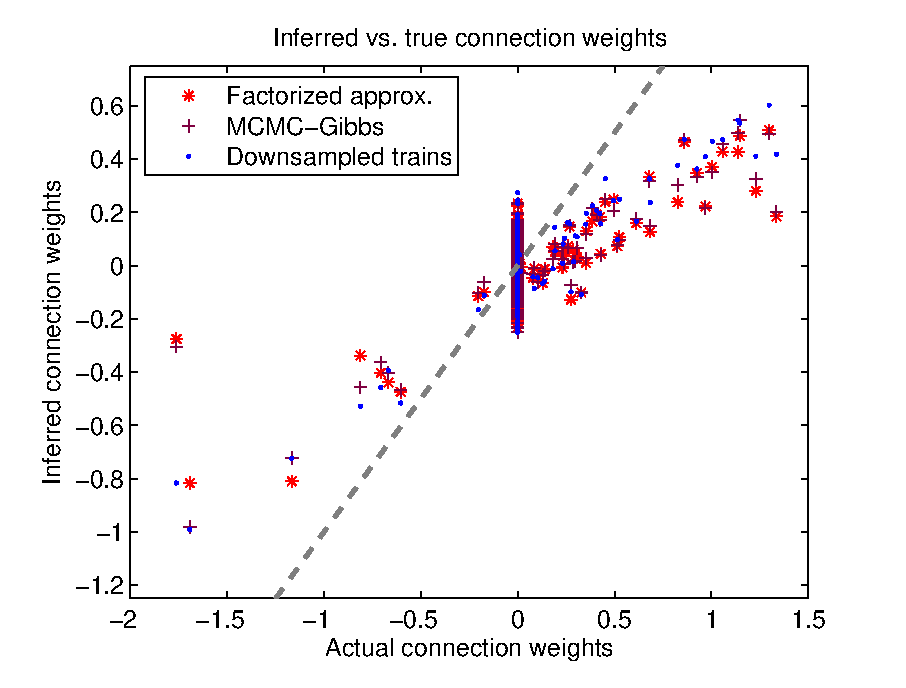
\includegraphics[width=\hsize]{../figs/FigureA3_scatter_three}
\end{minipage}
\begin{minipage}[c]{0.45\hsize}
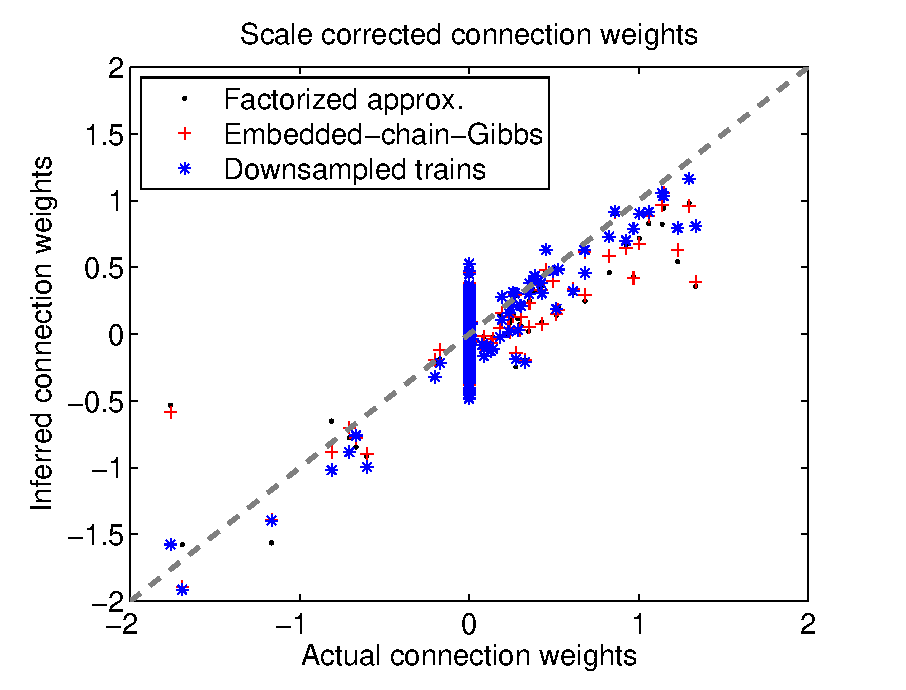
\includegraphics[width=\hsize]{../figs/FigureA3_scatter_three_corrected}
\end{minipage}
\caption{Functional connectivity matrix can be reconstructed from calcium imaging data.
Inferred connection weights are shown in a scatter plot versus real connection weights, with inference performed using factorized approximation, exact embedded-chain-within-blockwise-Gibbs approach, and true spike trains observed at the frame rate of the calcium imaging. Network of $N=25$ neurons was used, firing at $\approx 5$ Hz, and imaged for T=600 sec at intermediate SNR (photon budget 10Kph/neuron/frame, see below). $r^2=0.47$ for factorized approximation, $r^2=0.48$ for embedded-chain-within-blockwise-Gibbs, and $r^2=0.57$ for true down-sampled spike trains. Factorized approximation produced results almost as accurate as the exact embedded-chain-within-blockwise-Gibbs approach, and almost as accurate as the original spikes. Inferred connectivity weights were always scaled with respect to true connectivity due to time discretization bias (see main text).
This bias can be successfully calculated theoretically and removed from
the estimate of $\bw$.} \label{fig:scatters} \end{figure}

\subsection{Impact of coarse time discretization of calcium imaging data and scale bias in inferred connection weights}
Spike trains, necessary to evaluate functional connectivity matrix $\bw$, here were inferred with discretization into time-bins corresponding to the frame-rate of calcium imaging fluorescence data. In principle, one could use super-resolution feature of \cite{Vogelstein2009} to obtain spike trains with arbitrarily small time step $\Delta\rightarrow 0$. However, the problem in that case is that the spikes, inferred from fluorescence data, contain inaccuracy in their temporal position $\approx 1/$frame-rate,  due to the time-discretization of the underlying fluorescence trace.
Thus, when we super-resolve spikes using \cite{Vogelstein2009}, the spike pairs such that a spike of neuron $i$ closely follows a spike of neuron $j$ can be often confused with such where a spike of neuron $j$ closely follows a spike of neuron $i$.
It, therefore, becomes impossible to determine which neuron fired first, and which neuron
was pre-synaptic or post-synaptic in given pair of neurons $i$, $j$.
More specifically,
%because we rely on empirically counting close spike pairs in a set of spike trains to estimate the spike-triggered probabilities for spikes of different pairs of neurons, $i$ and $j$, which then allow estimating $w_{ij}$, above disordering of close spike pairs results in dramatic noise component in our estimate for the functional connectivity matrix by not allowing to effectively distinguish $w_{ij}$ and $w_{ji}$.
when using $\Delta \rightarrow 0$, we observed large errors in $\bw$,
$var[\bw] \propto \bw + \bw^T$ - because of inaccuracies in temporal position of spikes inferred from calcium imaging it became impossible to reliably distinguish which neuron causally preceded which other neuron, and only a-causal connectivity matrix $(\bw + \bw^T)/2$ could be determined.

To circumvent this problem, we (down-)sampled the time-axis in bins of size $\Delta=1/$frame-rate, and treated all spike pairs that occurred within the same time-bin as coincidental. This successfully counteracted the above problem and, additionally, allowed to perform calculations substantially faster by using larger $\Delta$. At the same time, this resulted in scale bias that all our inferred  connectivity matrices consistently exhibited, Figure \ref{fig:scatters}. This bias may be successfully understood and corrected from the following time-discretization argument.
Specifically, estimating the magnitude of the connection weight $w_{ij}$ is based on empirically evaluating the spike-triggered probability of neuron $i$ to fire, conditioned on neuron $j$. Most significant change in the spiking probability of neuron $i$, conditioned on neuron $j$, occurs within $\tau_w \approx 10-20$ msec from a spike of neuron $j$.
%To evaluate the magnitude of weight $w_{ij}$, therefore, we evaluate how many pairs of spikes, comprised of a spike of neuron $i$ following spike of neuron $j$ within $\approx \tau_w$, were empirically observed in a given spike train, and what spike-triggered probability this corresponds to.
When spike trains are down-sampled into large time-bins, e.g. $\Delta = 30$ msec, a significant fraction of close spike pairs appears coincident and not causal, as both spikes from neuron $i$ and neuron $j$ within $\approx \tau_w$ from each other are often assigned to the same time-bin.
As we discussed in the previous paragraphs, such close spike pairs typically introduce a great deal of noise in the estimate of $\bw$.
When $\Delta$ is large, however, most of such unreliable spike pairs would be considered coincidental and would not affect $\bw$ estimate. At the same time, all of such close pairs would be lost if we were to empirically evaluate the spike-triggered probabilities, which would have led us to believe in a lower than the actual  $w_{ij}$.


%
% Really, if the number of spikes of one neuron following that of another neuron within $\Delta$ was $n(2\rightarrow 1)$, while such in the reverse order was $n(1\rightarrow 2)$, difference $\delta n_{12} = n(2\rightarrow 1)-n(1\rightarrow 2)$ would correspond to the difference of functional connectivity weights $\delta w_{12}=w_{12}-w_{21}$. However, when such spike pairs had had their order confused with large probability $p\approx 1/2$, the number of spike pairs $n(2\rightarrow 1)$ actually observed would become $(1-p) n(2\rightarrow 1)+p n(1\rightarrow 2)$, and similarly for the reverse. Empirically observed difference $w_{12}-w_{21}$ thus would correspondingly drop to $\delta w'_{12}= (1-2p)\delta w_{12}$, while the variance would remain the same.
% We observed that the amount of data necessary to overcome this noise due to disordering of closely positioned spike-pairs appeared to be well over $\approx 10$ min of data used for the most of the calculations shown in this section below. Such high-time-resolution samples of spike trains also were substantially more computationally expensive to obtain and work with. For these reasons, we did not pursue this line of research further, although it may be of interest in the future.

To estimate the magnitude of this time-discretization bias quantitatively, we consider a significantly simplified case of two neurons coupled with a small weight $w_{12}$, and firing with baseline firing rate of $r=f(b)=\exp(b)$, $b \gg w_{12}$.
A sufficient statistics for estimating $w_{12}$ in this case is, e.g.:
\begin{equation}\label{eqn:scale:leadin-1}
\begin{array}{rl}
S =& E\left[\int\limits_{t'}^{t'+\mathcal{T}} \text{dt} n_1(t) | n_2(t')=\text{spike}, n_2(t)=\text{no spike}\ \forall t'<t<t'+\mathcal{T}\right] \\
\approx & r \mathcal{T} + f'(b) \int^{\mathcal{T}}  \text{dt} w_{12} \exp(-t/\tau_w) \\
\approx & r \mathcal{T} + f'(b) w_{12}\tau_w,
\end{array}
\end{equation}
where $\tau_w \ll \mathcal{T} \ll 1/r$, and
\begin{equation}\label{eqn:scale:leadin-1}
w_{12}=(S-r\mathcal{T})/f'(b)\tau_w.
\end{equation}
Now, if the spike trains were down-sampled into time-bins of size $\Delta$,
we estimate statistics $S$ with a discrete sum:
\begin{equation}\label{eqn:scale:leadin-2}
\begin{array}{rl}
S^{ds}=&E\left[\sum\limits_{t=t'+\Delta}^{t'+\Delta + \mathcal{T}} n^{ds}_1(t) | n^{ds}_2(t')=1, n^{ds}_2(t)=0\ \forall
t'<t<t'+\mathcal{T}\right]. \\
\approx& r \mathcal{T} + f'(b) \int\limits_0^\Delta \frac{\text{dt}'}{\Delta} \int\limits_{\Delta}^{\Delta + \mathcal{T}} \text{dt} w_{12}\exp(-(t-t')/\tau_w) \\
\approx & r \mathcal{T} +  f'(b)w_{12}\frac{1-\exp(-\Delta/\tau_w)}{\Delta/\tau_w^2}.
\end{array}
\end{equation}
$n^{ds}(t)$ here are down-sampled spikes, i.e. the spikes defined on a grid $t=0,\Delta,2\Delta,\ldots$.
In the second equality we took into account that the true position of the spike of the second neuron, $n^{ds}_2(t')$, may be uniformly distributed in first time-bin, here $[0,\Delta]$, and discrete sum over $t$ is from second time-bin $[\Delta,2\Delta]$ to $[\mathcal{T},\mathcal{T}+\Delta]$, i.e. over all spikes of the first neuron that occurred in any of the strictly subsequent time-bins up to $\mathcal{T} + \Delta$.
If we were to naively apply GLM Eq. \ref{eqn:scale:leadin-1} here using down-sampled estimate $S^{ds}$, we would have obtained
\begin{equation}\label{eqn:bias}
w_{12}^{ds}\approx \frac{1-\exp(-\Delta/\tau_w)}{\Delta/\tau_w} w_{12}.
\end{equation}
This is the scale bias that we observe.
In Figure \ref{fig:bias} we plot the scale bias from Eq. \ref{eqn:bias} versus that empirically deduced from our simulations for different values of $\Delta$. As can be seen in Figure \ref{fig:bias}, Eq. \ref{eqn:bias} describes observed scale bias very well.

\begin{figure}[h]
\centering
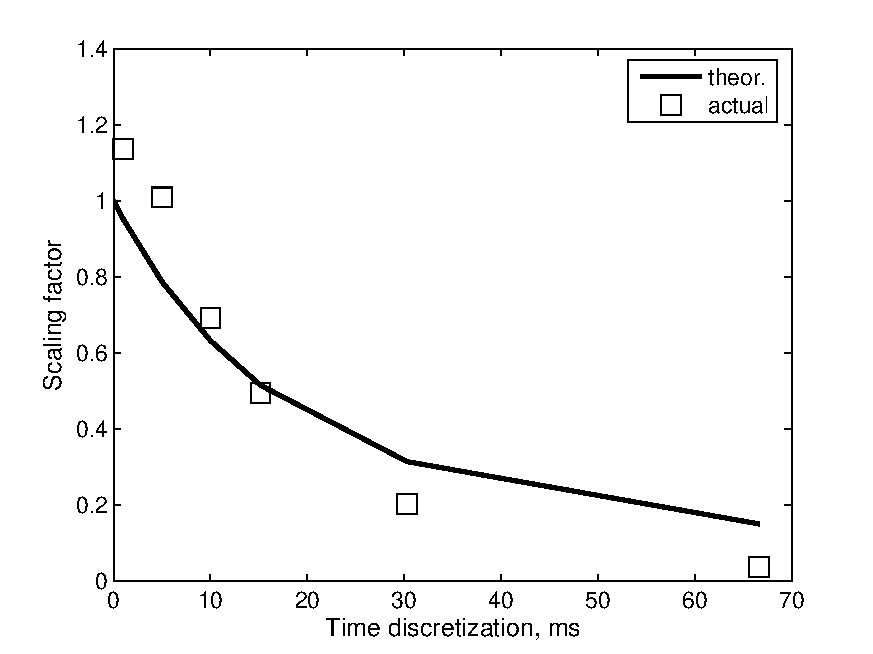
\includegraphics[width=3in]{../figs/FigureA4_scale_bias}
\caption{The low-frame rate of calcium imaging can explain the scale bias in inferred connectivity weights in Figure \ref{fig:scatters}.  Theoretically, scale bias may be evaluated by calculating what fraction of spikes from two neurons would occur within a single time-bin of width $\Delta$ (c.f. Eq. \ref{eqn:bias}).
Plotted such theoretically calculated scale bias (line) vs. that observed empirically from our simulations (box), from a simulation of $N=25$ neurons, $T=10$ min.
The error-bars correspond to 95\% confidence intervals for scale bias estimate.}
\label{fig:bias}
\end{figure}

\subsection{Impact of using priors on the inference}

\begin{figure}[h]
\centering
\begin{minipage}[c]{0.45\hsize}
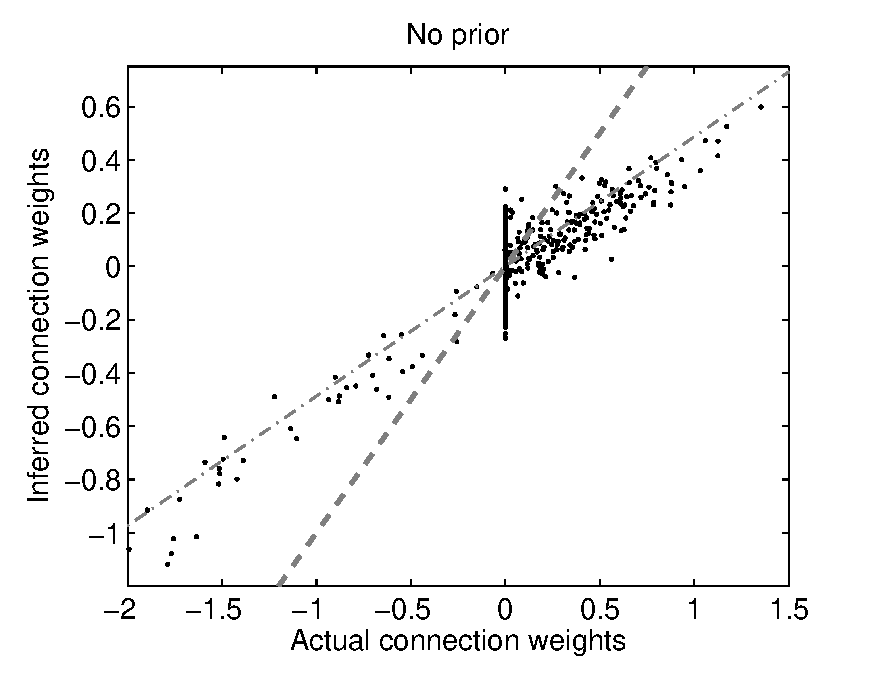
\includegraphics[width=\hsize]{../figs/FigureA10_regular_sol}
\end{minipage}
\begin{minipage}[c]{0.45\hsize}
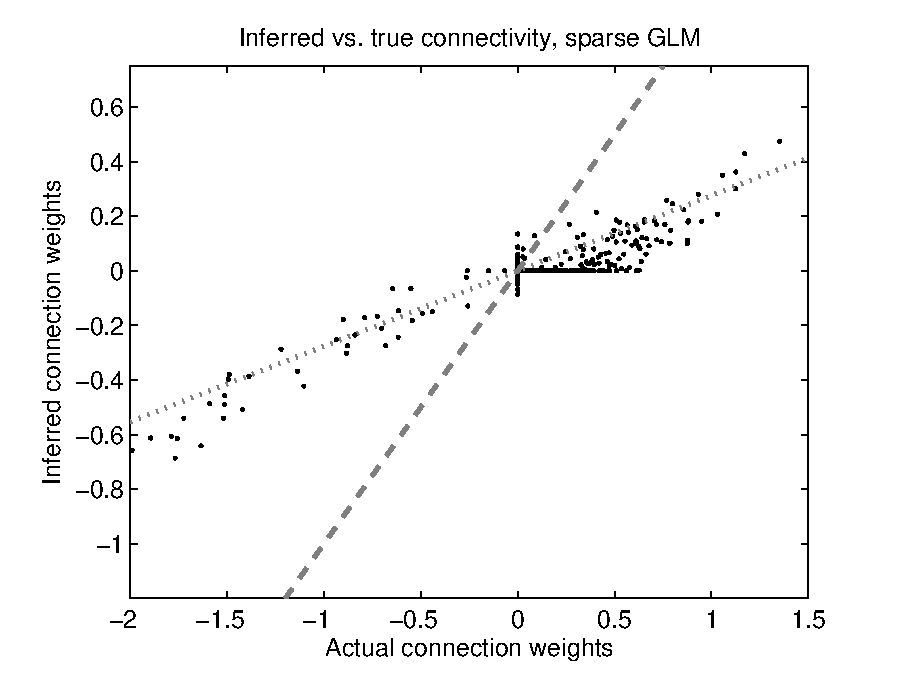
\includegraphics[width=\hsize]{../figs/FigureA10_sparse_sol}
\end{minipage}
\caption{
Incorporating simple priors on the distribution of connectivity weights, such as exponential sparseness prior, is essential to achieve much more accurate reconstructions from a smaller amount of calcium imaging data.
Shown here are the connection weights reconstructed using GLM (left panel) or sparse-prior GLM (right panel) are shown in a scatter plot for a network of $N=50$ neurons, firing at $\approx 5$ Hz, and imaged for $T=600$ sec. $r^2=0.64$ for simple GLM and $r^2=0.85$ for sparse-GLM.
Since original $\bw$ is sparse, noise in the estimates of $w_{ij}=0$ results in a vertical line at zero in the left panel.
Likewise, sparse prior results in many small $w_{ij}$ to be deduced as zeros, which produces the horizontal line at zero in the right panel.
}
\label{fig:sparse}
\end{figure}

\begin{figure}[h]
\centering
\begin{minipage}[c]{0.45\hsize}
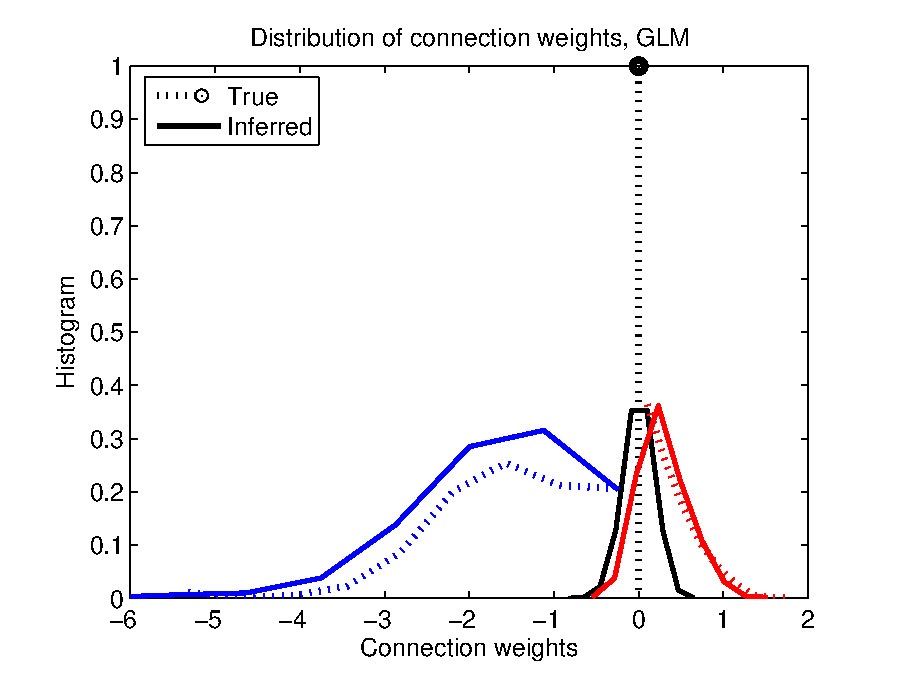
\includegraphics[width=\hsize]{../figs/FigureA3_hist_glm200}
\end{minipage}
\begin{minipage}[c]{0.45\hsize}
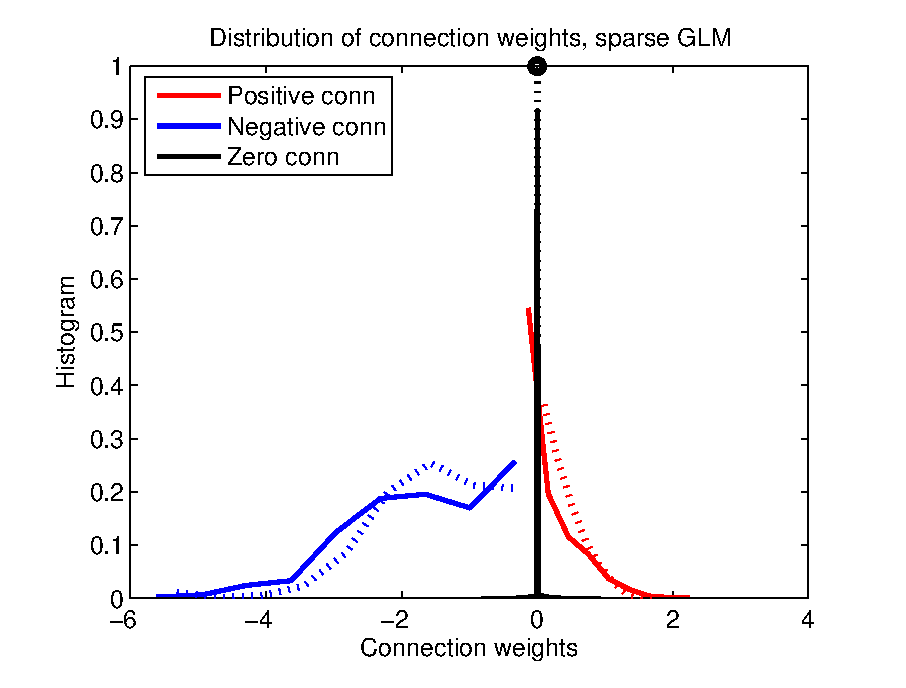
\includegraphics[width=\hsize]{../figs/FigureA3_hist_spa200}
\end{minipage}
\caption{
The distribution of inferred connection weights using GLM (left) and sparse GLM (right) vs. true distributions. When sparse exponential prior is enforced, dispersion in inferred connection weights is substantially reduced and, in particular, it becomes possible to reliably determine which neural pairs are connected, and which neurons are excitatory or inhibitory. Distributions are shown for a network of $N=200$ neurons, firing at $\approx 5$ Hz, and imaged for $T=600$ sec.}
\label{fig:distros}
\end{figure}


Taking into account simple prior information about the connectivity matrix results in dramatic improvement of the inferred connectivity matrix, Figure \ref{fig:sparse} and \ref{fig:distros}, allowing successful reconstruction from as little as 5 min of calcium imaging data, and for $T\approx 10$ min achieving the same level of accuracy otherwise requiring up to $T\approx 1$ hour of calcium imaging, Figure \ref{fig:recvar-NT}.
For example, in a network of $N=50$ neurons imaged for $T=10$ min, $r^2$ is increased from $r^2=0.64$ to $r^2=0.85$ when sparse prior was enforced.
Furthermore, $\bw$ estimates calculated with sparse prior allow reliable determination which neurons are connected, or which neurons are inhibitory or excitatory in nature, Figure \ref{fig:distros}.
At the same time, sparse prior introduces additional scale bias into connectivity estimates, which, therefore, effectively destroys information about the true scale of the connection weights.
Dale's prior, on the other hand, only leads to ~10\% in the correlation coefficient $r^2$ of the reconstructed connectivity matrix, and was not found significant. In case when sparse prior was initially enforced, enforcing Dale's prior typically resulted in no improvement to $\bw$ at all.


\subsection{Impact of different imaging frame rates, noise levels, and durations on the estimator accuracy}

\begin{figure}[h]
\centering
\includegraphics[width=3in]{../figs/FigureA5_recvar}
\caption{Accuracy of the inferred connectivity as function of the frame rate of calcium imaging. Connectivity matrix here was inferred from the original spike trains observed at corresponding frame rates, thus establishing the upper performance bound on the inference from calcium imaging data. A network of $N=25$ neurons, firing at $\approx 5$ Hz and imaged for $T=600$ sec was to generate this plot.}
\label{fig:recvar}
\end{figure}

\begin{figure}[h]
\centering
\begin{minipage}[c]{0.6\hsize}
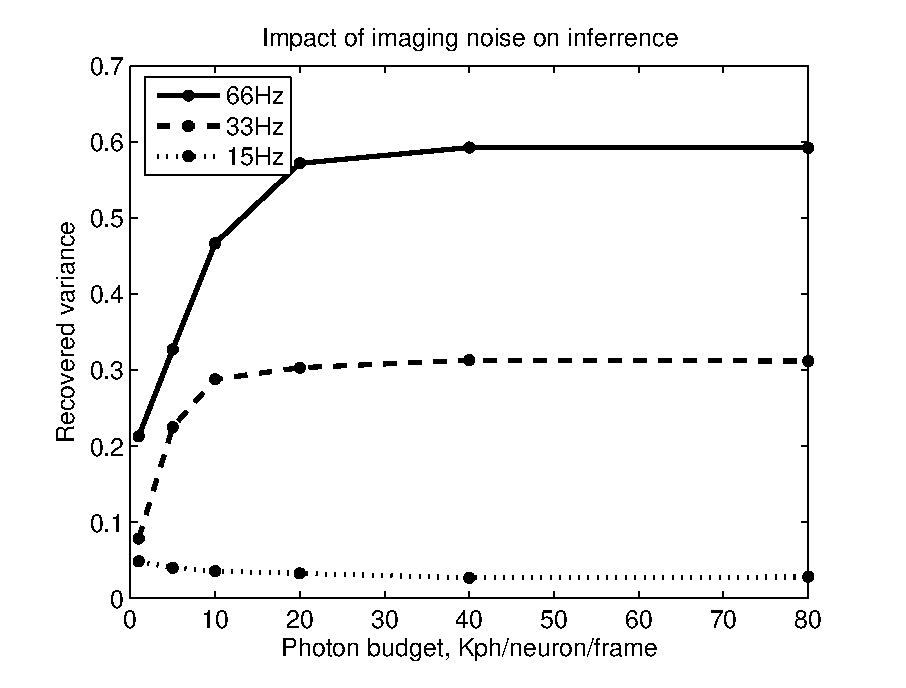
\includegraphics[width=\hsize]{../figs/FigureA6_recvar_SNR}
\end{minipage}
\begin{minipage}[c]{0.45\hsize}
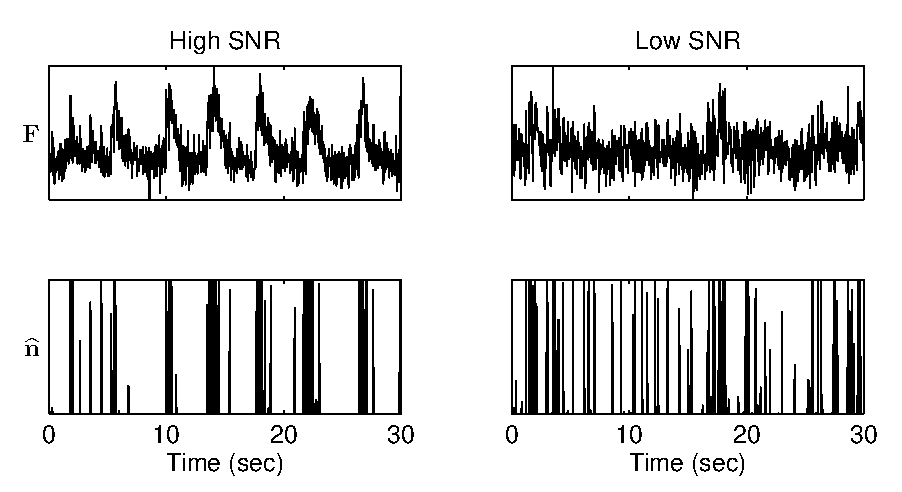
\includegraphics[width=\hsize]{../figs/example_traces}
\end{minipage}
\begin{minipage}[c]{0.45\hsize}
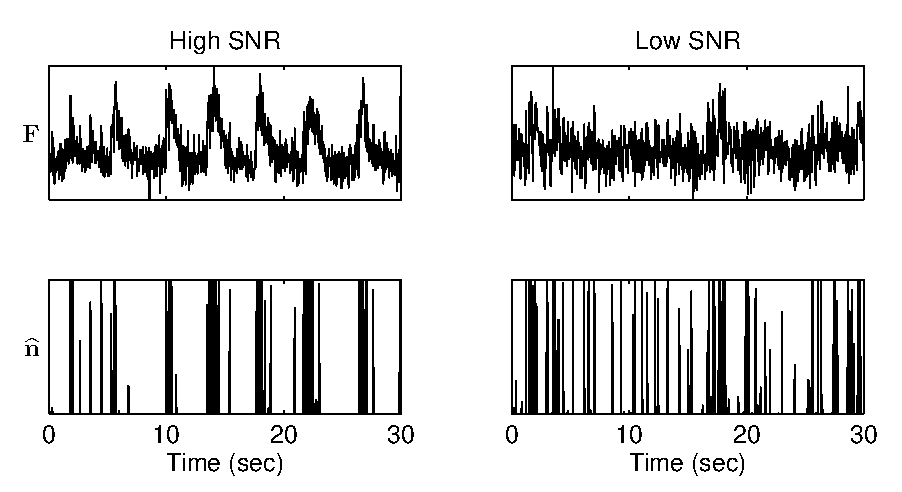
\includegraphics[width=\hsize]{../figs/example_traces}
\end{minipage}
\caption{Accuracy of inferred connectivity as function of the noise amount in the calcium imaging data, as quantified by photon budget, per neuron-frame, for frame rates of 15 Hz, 33 Hz and 66 Hz. Photon counts on the order of 10-20 Kph/frame/neuron are required to achieve the upper bound due by the frame rate. Connectivity matrix here was inferred from simulated fluorescence data using factorized approximation algorithm. Simulation conditions are the same as in Figure \ref{fig:recvar}.  Vertical black lines correspond to the two example traces in the lower panels, left to right respectively.}
\label{fig:recvar-SNR}
\end{figure}

\begin{figure}[h]
\centering
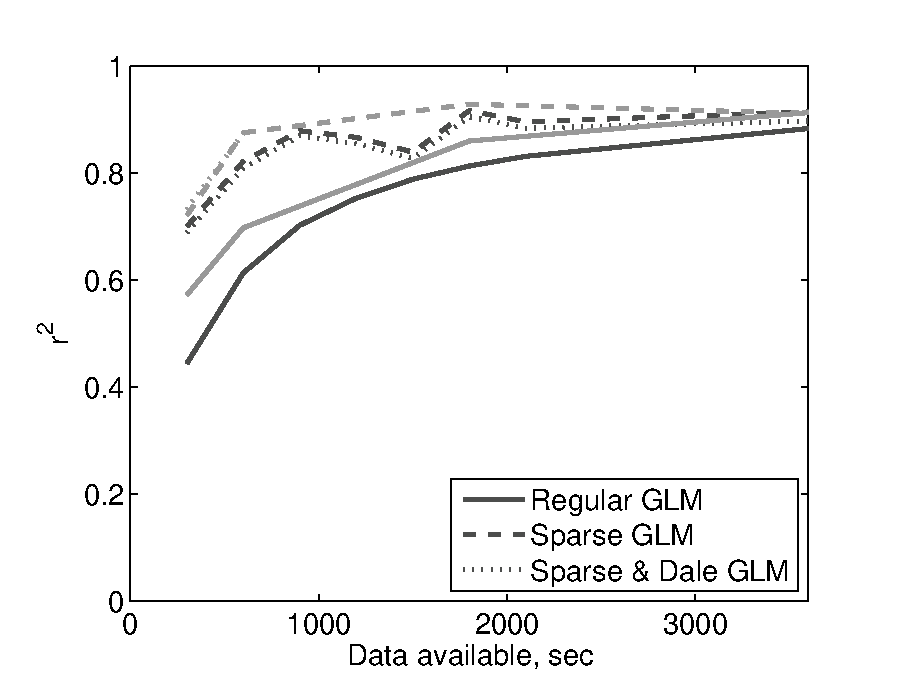
\includegraphics[width=3in]{../figs/FigureA7_recvar_NT}
\caption{Accuracy of inferred connectivity as function of the imaging time and neural population size. Incorporating simple priors such as exponential sparseness prior allows to boost dramatically the reconstruction's quality (dashed lines). In this latter case, $T=300$ sec is already sufficient to recover 70\% of the variance in the connection weights. Incorporating Dale's prior leads to only marginal improvement (dotted line). As shown in the methods, reconstruction accuracy does not depend on the neural population size $N$.
Here, neural population from $N=10$ to $N=200$ were simulated for different $T$, where
$N=200$ (gray) and $N=100$ (black) are shown. All networks were prepared in similar state by adjusting strength of inhibitory connections to achieve similar mean firing rate $\approx 5$ Hz, although actual firing rate could vary.
}
\label{fig:recvar-NT}
\end{figure}


What minimal conditions for the experimental setup should be met to allow successful reconstruction of the connectivity from calcium imaging data? In Figures \ref{fig:recvar} -- \ref{fig:recvar-NT} we address this question. Figure \ref{fig:recvar} shows the quality of the inferred connectivity matrix as function of the imaging frame rate - imaging frame rates 30-60 Hz are needed to achieve meaningful reconstruction results.
Frame rates $\approx 100$ Hz allow achieving the same level of the connectivity matrix reconstruction that is possible with the exact knowledge of the true spike trains.
Imaging frame 30-60 Hz are already possible in existing experimental setups, and imaging
at 100 Hz may be technologically possible in the future \cite{NguyenParker01,ReddySaggau05,Iyer06,SalomeBourdieu06,ReddySaggau08}

Figure \ref{fig:recvar-SNR} shows the quality of the inferred connectivity matrix as function of effective SNR and photon budget. Operationally, we define effective SNR as
\begin{equation}
eSNR=\frac{E[F_i(t)-F_i(t-1)|n_i(t)=1]}{E[{(F_i(t)-F_i(t-1))^2}/{2}|n_i(t)=0]^{1/2}},
\end{equation}

\noindent and photon budget as $\gamma^{-1}$. Photon budget corresponds to the number of photons collected from single neuron within a single frame, at the peak of fluorescence intensity. From our experience with the analysis of real cells \cite{Vogelstein2009}, the eSNR in real data was $\sim 3$ for in vivo data collected at 15  Hz and $\sim 9$  for in vitro data at the same frame rate. As can be seen from Figure \ref{fig:recvar-SNR}, the effective SNR necessary for accurate reconstructions was $\approx 5$. This eSNR corresponded to photon budgets of $\approx 10$ Kph/neuron/frame.
For lower eSNR, the amount of noise in calcium imaging data degraded inferred connectivity matrices significantly.

Finally, Figure \ref{fig:recvar-NT} shows the quality of the inferred connectivity matrix as function of the experiment duration. The minimal amount of data for a particular $r^2$ depended substantially on whether priors were enforced in M-step. In particular, for the M-step lacking a sparse prior, the calcium imaging duration necessary to achieve $r^2=0.5$ for the reconstructed connectivity matrix was $T\approx 10$ min, and $r^2=0.75$ was achieved at $T\approx 30$ min. When M-step enforced sparseness prior, $r^2>0.7$ was achieved already at $T\sim 5$ min. Furthermore, we observed that the accuracy of the reconstruction did not deteriorate with the size of the imaged neural population, whereas the same reconstruction quality was observed with the same amount of data for $N=50-200$ neurons.
This, at first unexpected, result is the direct consequence of the structure of the covariance matrix for $\bw$, as will be discussed below.
In all cases, good reconstructions were possible to obtain with only $T\sim 5$--$30$ min of calcium imaging data.


\subsection{Accuracy of the estimates and Fisher information matrix} \label{sec:methods:accuracy_Fisher}

Here we calculate theoretically the amount of spike trains data necessary to accurately estimate the functional connectivity matrix $\bw$. For clarity, we assume here that $\Delta \rightarrow 0$, and so $f(J)\approx e^J\Delta$, and that the spike trains are known perfectly, i.e. there is no corruption due to inference from low-SNR calcium imaging data.
As we shown above, for sufficient SNR this latter condition can be certainly achieved by calcium imaging data.
We also assume that the spikes only couple over a single time bin, i.e. $h_{ij}(t)\equiv n_j(t-\Delta)$.
Then, using GLM likelihood
\begin{equation}\label{eqn:fisher-glm}
\begin{array}{rl}
-\ln P[\bw | \bX] &\sim -\ln P[\bX | \bw] =
\sum\limits_{i,t} \left[ n_i(t) \ln f(J_i(t)) + (1-n_i(t)) (1-f(J_i(t))) \right], \\
J_i(t) &= b_i(t) + \sum\limits_j w_{ij} h_{ij}(t), \\
h_{ij}(t) &= n_j(t-\Delta),
\end{array}
\end{equation}
the Fisher information matrix for $P[\bw | \bX]$ is:
\begin{equation}\label{eqn:fisher-def}
\begin{array}{rl}
C^{-1}_{ij;i'j'}=\left[\frac{\partial (-\ln P[\bw | \bX])}{\partial \w_{ij}\partial \w_{i'j'}}\right]
=-&\delta_{ii'}\sum\limits_t\left[
n_i(t)n_{j}(t-\Delta)n_{j'}(t-\Delta)\left(-\frac{f'(J_i(t))^2}{f(J_i(t))^2} +
\frac{f''(J_i(t))}{f(J_i(t))}\right) - \right. \\
&\left.-(1-n_i(t))n_{j}(t-\Delta)n_{j'}(t-\Delta)f''(J_i(t))\right].
\end{array}
\end{equation}
where $f'$ and $f''$ correspond to the first and the second derivatives of our linking function (c.f Eq. \ref{eqn:glm:definition}), and $\delta_{ii'}$ is
the Kronecker's delta symbol, $\delta_{ii'}=1$ for $i=i'$, and $\delta_{ii'}=0$ otherwise.  Letting $f(J)=e^J\Delta$, the first term in the sum in Eq. \ref{eqn:fisher-def} cancels out, and the rest may be rewritten as:
\begin{equation}\label{eqn:fisher}
\begin{array}{rl}
C^{-1}_{ij;i'j'}
&=\delta_{ii'} T P[n_i(t)=0, n_j(t-\Delta)=1, n_{j'}(t-\Delta)=1]\times \\
&\times E[e^{J_i(t)}|n_i(t)=0, n_j(t-\Delta)=1, n_{j'}(t-\Delta)=1] \\
&= \delta_{ii'}T\left[(r \tau_w)\delta_{jj'}+O((r \tau_w)^2)\right]r.
\end{array}
\end{equation}
Here, $TP[n_i(t)=0, n_j(t-\Delta)=1, n_{j'}(t-\Delta)=1]$ describes the number of nonzero
terms in Eq. \ref{eqn:fisher-def}, corresponding to the condition that
$(1-n_i(t))n_{j}(t-\Delta)n_{j'}(t-\Delta)$ is only nonzero when
$n_i(t)=0, n_j(t-\Delta)=1, n_{j'}(t-\Delta)=1$.
$r=E[e^{J_i(t)}|n_i(t)=0, n_j(t-\Delta)=1, n_{j'}(t-\Delta)=1]$, then,
corresponds to the average value of $f''(J_i(t))$, conditional on such nonzero events.
$r\tau_w \ll 1$ is the probability for a neuron to spike over the time-interval  $\tau_w$.

The Fisher information matrix is block-diagonal, $C^{-1}_{ij;i'j'} \propto \delta_{ii'}$,
due to the structure of the log-likelihood $P[\bX | \bw]$, in particular, that it is represented as a sum over $i$ of independent terms, Eq. \ref{eqn:fisher-glm}.
But also from Eq. (\ref{eqn:fisher}) we observe that Fisher information matrix is predominantly diagonal, $C^{-1}_{ij;i'j'} \propto \delta_{ii'}\delta_{jj'}$, and thus the covariance matrix $C$can be computed trivially:
\begin{equation}
C = (rT)^{-1} (r \tau_w I + O((r \tau_w)^2))^{-1} =
(r^2 \tau_w T)^{-1} I + O((r \tau_w)^2)
\end{equation}

For successful determination of the functional connectivity matrix $\bw$, the variance $C$ should be made smaller than the typical scale $\langle \bw^2\rangle$, thus:
\begin{equation}
T \sim (\langle \bw^2 \rangle r^2  \tau_w)^{-1}.
\end{equation}
For typical values of $\bw^2\approx 0.1$, $r\approx 5$  Hz and $ \tau_w \approx 10$ msec,
with this order of magnitude estimate we obtain $T$ of the order of hundred seconds. This theoretical estimate of the necessary amount of fluorescent data is in good agreement with our simulations.

Finally, because $C^{-1}$ is diagonal, this scale of $C$ does not depend on the number of neurons in the imaged neural population, $N$. Thus, the variance of the estimate $\bw$ does not degrade with the size of the imaged population, $N$, for the same amount of data, $T$.

\subsection{Impact of strong correlations and deviations from generative model on the inference}

%Fig 7: non-robustness to strong correlations
%top panels: rasters
%bottom panels: corrected scatter plots
%
\begin{figure}[h]
\centering
\begin{minipage}[c]{0.45\hsize}
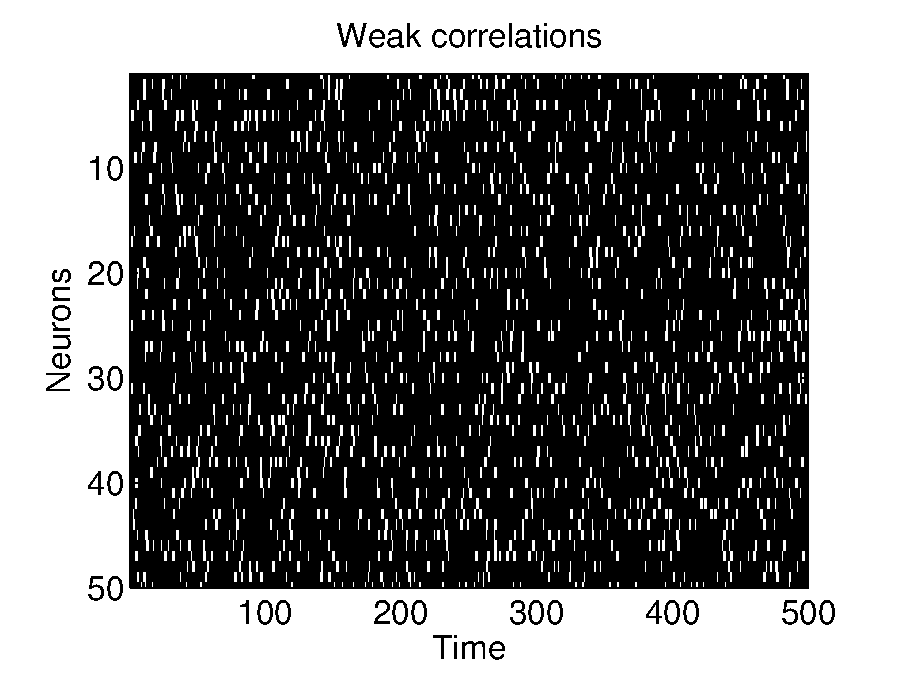
\includegraphics[width=\hsize]{../figs/Figure7b_raster_weak}
\end{minipage}
\begin{minipage}[c]{0.45\hsize}
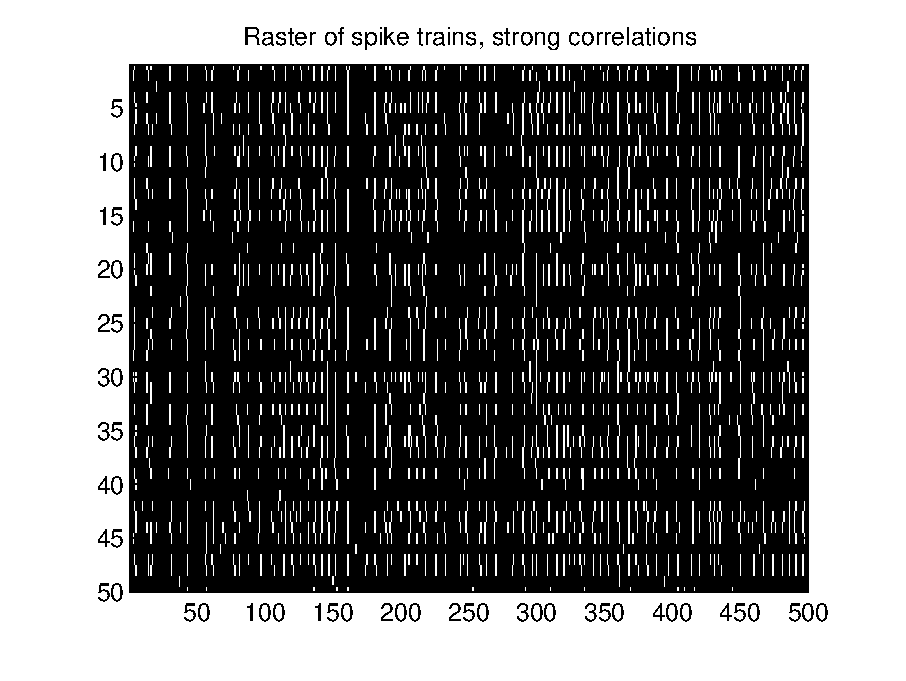
\includegraphics[width=\hsize]{../figs/Figure7a_raster_strong}
\end{minipage}
\begin{minipage}[c]{0.45\hsize}
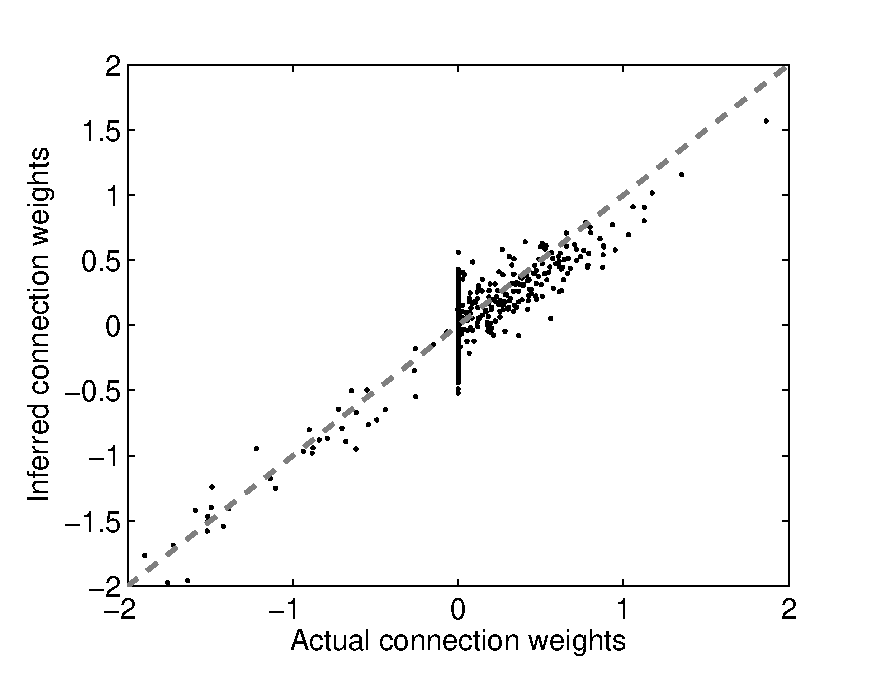
\includegraphics[width=\hsize]{../figs/FigureA8_weak_corr}
\end{minipage}
\begin{minipage}[c]{0.45\hsize}
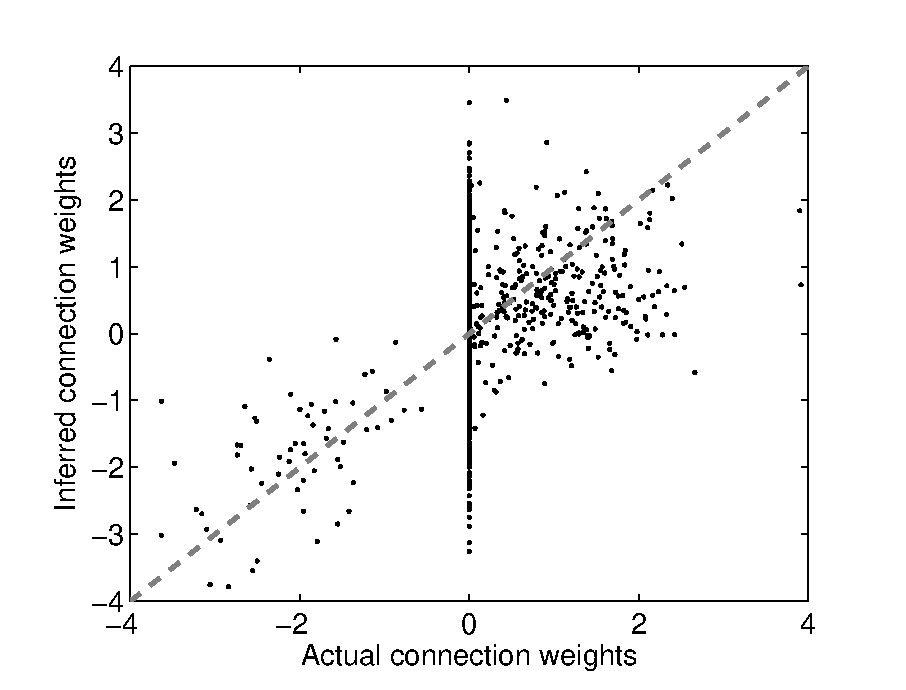
\includegraphics[width=\hsize]{../figs/FigureA8_strong_corr}
\end{minipage}
\caption{
Diverseness of observed neural activity patterns is required for
functional connectivity to give access to the actual ``anatomical'' structure
of the neural circuit. Here, 15 sec of simulated spike trains for a weakly coupled network (upper-left) and a network with strongly coupled component (upper-right) are shown.
In weakly coupled network spikes are sufficiently uncorrelated to give access to all different neural activity patterns needed to properly estimate true weights ${\bf w}_i$. In strongly coupled case, many instances of highly synchronous locked firings are evident, thus preventing observation of sufficiently rich ensemble of activity patterns.
Accordingly, GLM solution for the strongly coupled neural network (lower-right) does not
represent the true connectivity of the circuit, even for the weakly coupled component. This is contrary to the weakly-coupled network (lower-left) where true connectivity is successfully obtained.
Networks of $N=50$ neurons firing at $\approx 5$ Hz and imaged for $T=600$ sec were used to produce this figure.}
\label{fig:rasters}
\end{figure}

\begin{figure}[h]
\centering
\begin{minipage}[c]{0.45\hsize}
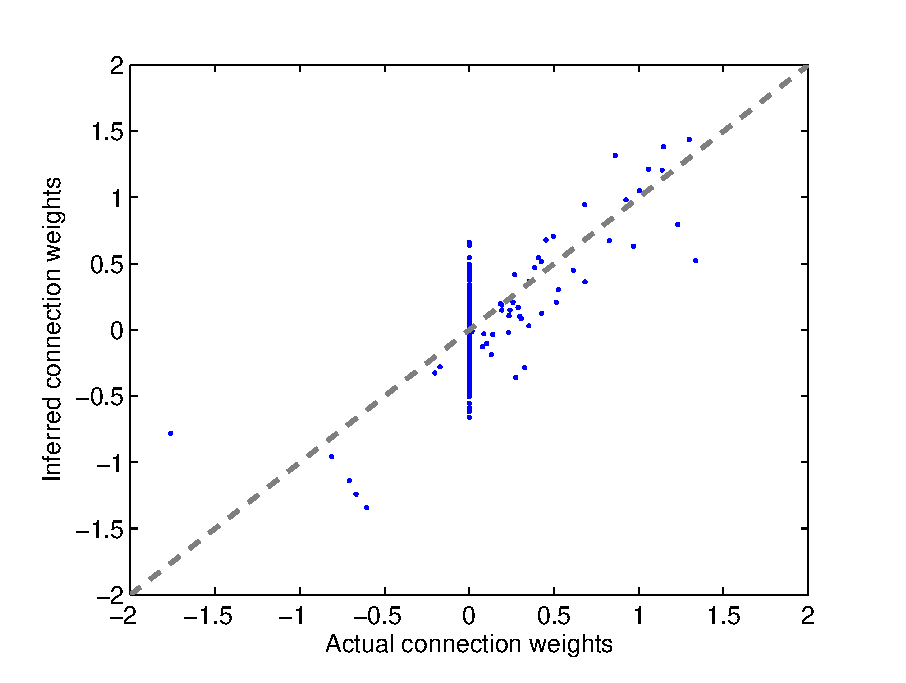
\includegraphics[width=\hsize]{../figs/FigureA9_all_same_sol}
\end{minipage}
\begin{minipage}[c]{0.45\hsize}
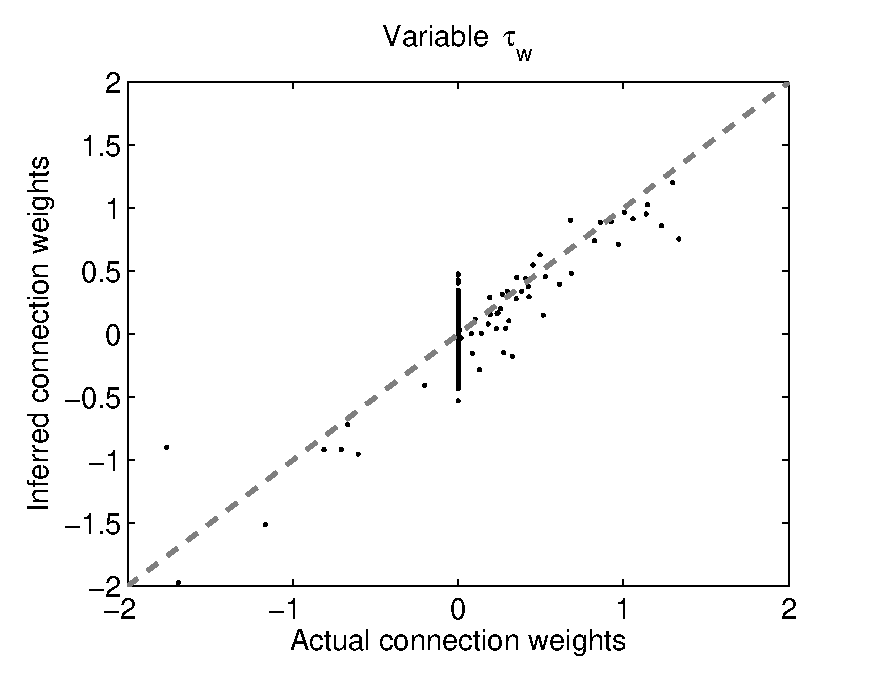
\includegraphics[width=\hsize]{../figs/FigureA9_variable_25}
\end{minipage}
\caption{Bayesian inference algorithm is robust to deviations of the
data from our generative model. One such deviation, that should be expected in real data, is variability in the EPSP time courses from neuron to neuron, and possibly synapse to synapse.
With up to 25\% variability allowed in EPSP time scales $\tau_w$ (right panel) our algorithm provided reconstructions of almost the same quality as when all $\tau_w$ were the same (left panel). Simulation conditions are the same as in Figure \ref{fig:recvar}.}
\label{fig:vartau}
\end{figure}


``Anatomical'' connectivity was recovered in our experiments despite potential problems noted in the literature [XXX], e.g. such as common input from correlated neurons. This is primarily due to the particular form of the activity in our neural networks, whereas firing of neurons occurred independently, thus, allowing GLM explore the full range of possible input configurations and disentangle common inputs.

Estimation of the functional connectivity is fundamentally routed in observing changes in the spike rate conditioned on the state of the other neurons. Intuitively, such estimation can be compared to observing changes in $f({\bf n}(t))\propto\exp(\sum_j \w_{ij}n_j(t))$ for different neural configurations ${\bf n}(t)$, i.e. estimating a vector ${\bf w}_i$ from a number of dot-products ${\bf w}_i\cdot {\bf n}(t)$. In order to properly estimate all components of ${\bf w}_i$ the set of available ${\bf n}(t)$ should be rich enough to span all $N$ dimensions of ${\bf w}_i$. In case of independent firing such condition is clearly satisfied.  Should this condition be violated, however, e.g. due to high correlation between spiking of few neurons, spike trains may not provide access to the true vector ${\bf w}_i$, and the connection weights inferred from such activity data may effectively ``aggregate'' true connection weights in arbitrary linear combinations.

We carried out a simulation of hypothetical ``strongly'' coupled  neural network, where in addition to weak sparse connectivity we introduced sparse random strong connectivity component. In a sense, we allowed a fraction of neurons to couple strongly to the other neurons, thus, making them ``command'' neurons ``driving'' the activity of the rest of the population. The strength of strong connectivity component was chosen to dynamically build up the actual firing rate from the baseline rate of $r=\exp(b)\approx 1$ Hz to $\approx 5$  Hz.
Such neural network showed patterns of activity very different from the weakly coupled networks inspected above, Figure \ref{fig:rasters}.  In particular, large number of highly correlated, synchronously locked firings of many neurons were evident in this network.  Likewise, our Bayesian algorithm was not able to identify the true connectivity matrix correctly, Figure \ref{fig:rasters}.

%Fig 8: robustness to variability in tau_h
%left: corrected scatter plot for (1) assuming same tau's, and (2) assuming they are all diff
%right: distributions of the weights, for truth and the above two approaches
%
%Fig 9: sparse glm improves fit (same format as Fig 8)
%




On the other hand, our inference algorithm showed significant robustness to deviations of the actual data from our generative model.
One important such deviation, which is likely to occur in the real experiments, is variation in the time-scales of EPSPs in different synapses. Up to now, all EPSP time-scales $\tau_w$ were assumed to be the same in our inference algorithm as well as in the simulations.
In Figure \ref{fig:vartau} we introduce additional variability in $\tau_w$ from one neuron to another.
Variability in $\tau_w$ results in added variance in the estimates of the connectivity weights $w_{ij}$ through $\tau_w$ dependence of the scaling factor Eq.(\ref{eqn:bias}).
Still, we found that such added variance was insignificant with $\tau_w$ varying for up to 25\% from neuron to neuron, Figure \ref{fig:vartau}.


%Fig -: real data
% \begin{figure}[h]
% \centering
% \begin{minipage}[c]{0.45\hsize}
% 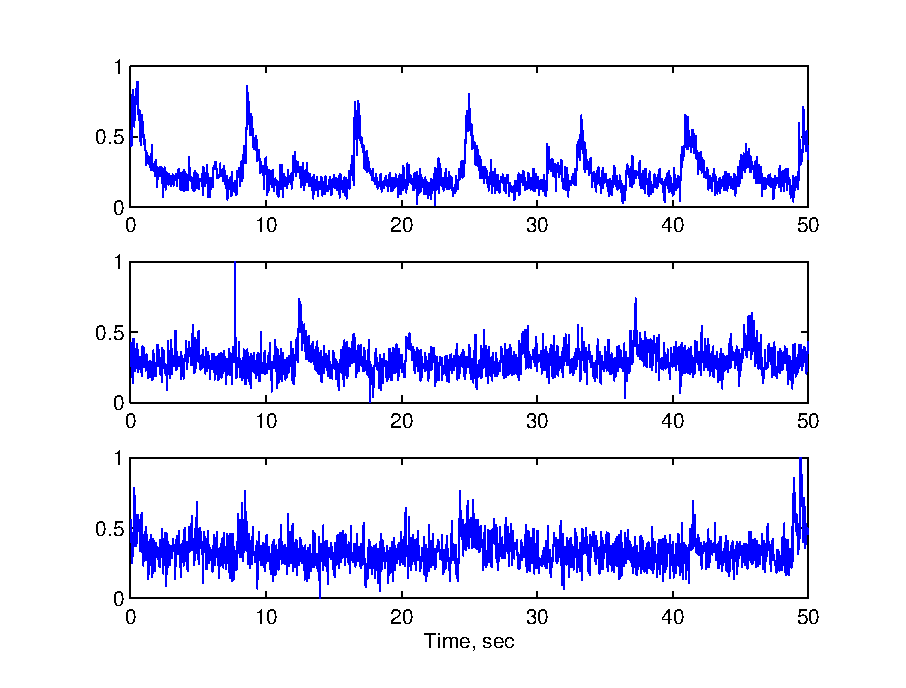
\includegraphics[width=\hsize]{../figs/FigureA11_real_traces}
% \end{minipage}
% \begin{minipage}[c]{0.45\hsize}
% 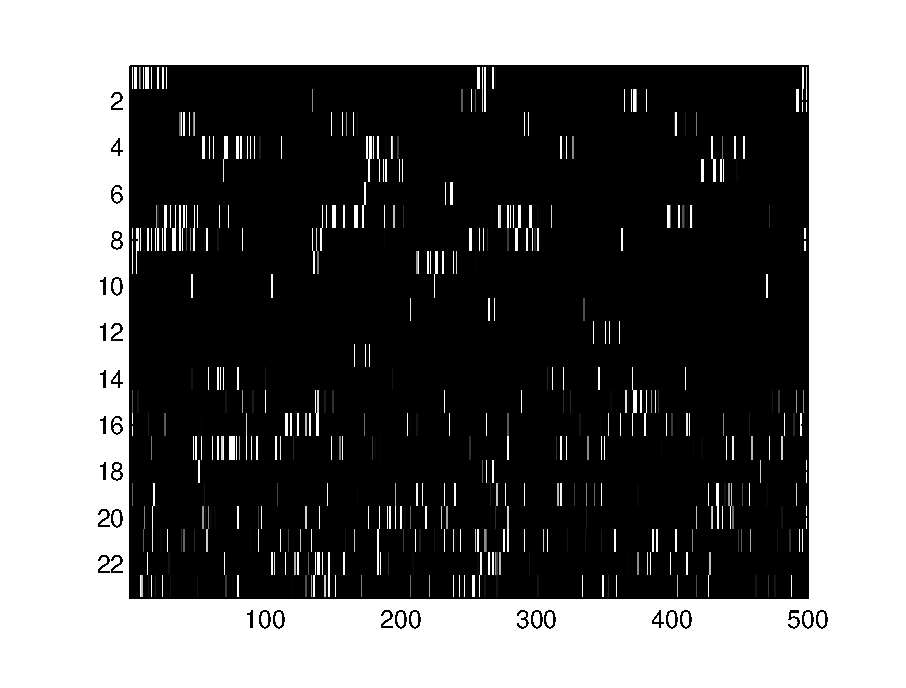
\includegraphics[width=\hsize]{../figs/FigureA11_real_raster}
% \end{minipage}
% \begin{minipage}[c]{0.3\hsize}
% 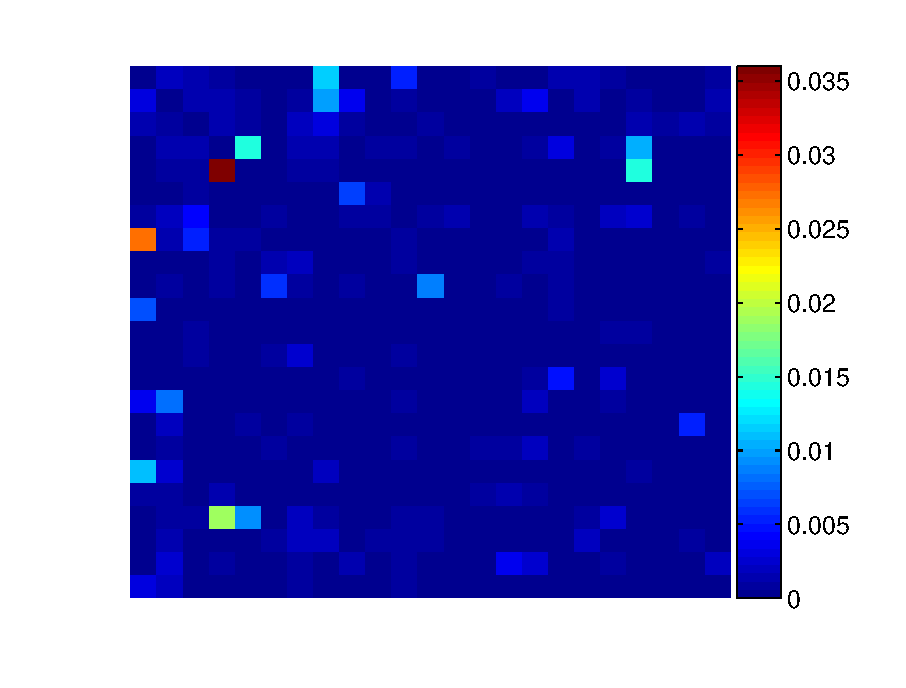
\includegraphics[width=\hsize]{../figs/FigureA11_real_Xcorr}
% \end{minipage}
% \begin{minipage}[c]{0.3\hsize}
% 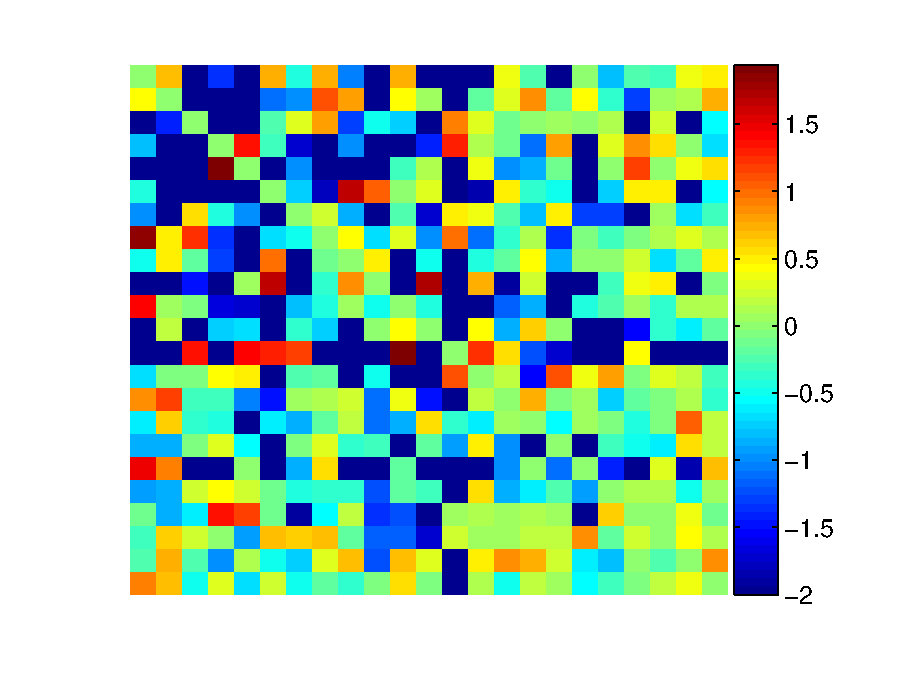
\includegraphics[width=\hsize]{../figs/FigureA11_real_glm}
% \end{minipage}
% \begin{minipage}[c]{0.3\hsize}
% 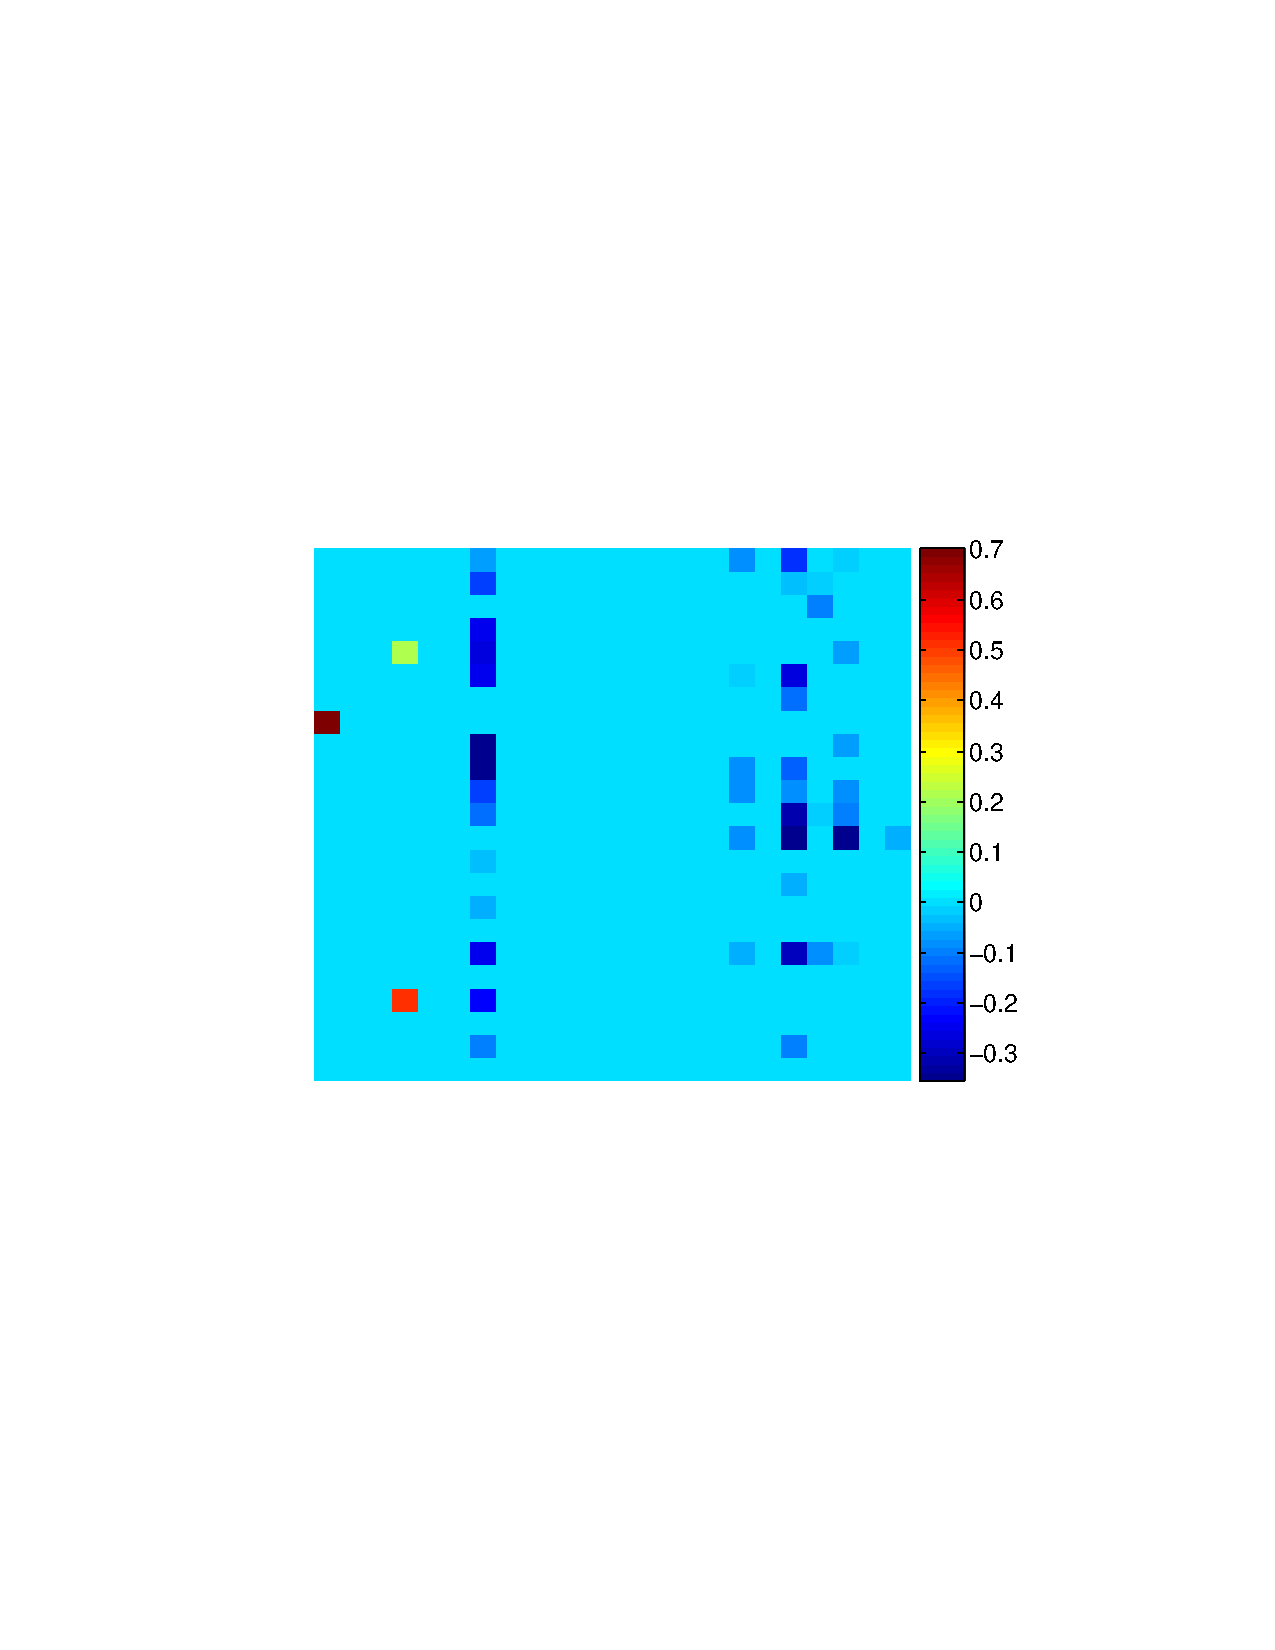
\includegraphics[width=\hsize]{../figs/FigureA11_real_sparse}
% \end{minipage}
% \caption{Functional connectivity matrix inferred from a sample of actual calcium imaging data for $N=72$ cells in [XXX], imaged for $T\approx 260$ sec at 15 Hz.
% $N=23$ neurons with spikes at sufficient SNR were selected, and functional connectivity reconstructed using factorized approximation algorithm. Firing cell of these cells was 0.1-1 Hz and 20-200 spikes were collected for each neuron.
% Upper-left panel shows example of actual fluorescence traces from selected cells, best to worst. Upper-right panel shows a raster of inferred spike trains for first 100 sec of imaging data. Lower panels show left-to-right the time-delayed cross-correlation matrix for selected neurons, simple GLM solution and sparse GLM solution, respectively. A consistent connectivity matrix is obtained here, with sparse solution having sparseness of $\approx 10 \%$, and all neurons automatically respecting Dale's law without explicitly enforcing it. Two clearly excitatory, and three clearly inhibitory neurons can be seen, with remaining neurons not showing significant couplings.}
% \label{fig:real}
% \end{figure}


%We applied our algorithm to a sample of the real calcium imaging data from [XXX], totaling about 5 minutes of imaging for a population of 72 cells in [XXX]. Out of these, about 23 cells had fluorescence traces indicative of spikes, while the other cells were either silent or did not shown SNR sufficient for analysis. These 23 cells were selected for futher processing. 20-200 spikes were found for each cell, corresponding to firing rates from 0.07 Hz to 0.8 Hz.
%We then identified functional connectivity matrix for this population. Sparse solution resulted in consistent connectivity matrix with sparseness of about 10\%, automatically respecting Dale's law, and clearly indicating two strongly connected excitatory neurons and few inihibitory neurons. Although this data lacked independent controls necessary to properly evaluate quality of our obtained reconstruction, it does demonstrate that our approach can be successfully applied under real-life condition to analyze functional connectivity of real populations of neurons.
